\documentclass[a4paper]{article}
\usepackage[pdftex]{hyperref}
\usepackage[latin1]{inputenc}
\usepackage[english]{babel}
\usepackage{a4wide}
\usepackage{amsmath}
\usepackage{amssymb}
\usepackage{algorithmic}
\usepackage{algorithm}
\usepackage{ifthen}
\usepackage{listings}
\usepackage{array}
\usepackage{tabu}
% move the asterisk at the right position
\lstset{basicstyle=\ttfamily,tabsize=4,literate={*}{${}^*{}$}1}
%\lstset{language=C,basicstyle=\ttfamily}
\usepackage{moreverb}
\usepackage{palatino}
\usepackage{multicol}
\usepackage{tabularx}
\usepackage{comment}
\usepackage{verbatim}
\usepackage{color}
\usepackage{graphicx}
\usepackage{array,mathtools}
\usepackage{amsmath}

%% pdflatex?
\newif\ifpdf
\ifx\pdfoutput\undefined
\pdffalse % we are not running PDFLaTeX
\else
\pdfoutput=1 % we are running PDFLaTeX
\pdftrue
\fi
\ifpdf
\fi
\ifpdf
\DeclareGraphicsExtensions{.pdf, .jpg}
\else
\DeclareGraphicsExtensions{.eps, .jpg}
\fi

\parindent=0cm
\parskip=0cm

\setlength{\columnseprule}{0.4pt}
\addtolength{\columnsep}{2pt}

\addtolength{\textheight}{5.5cm}
\addtolength{\topmargin}{-26mm}
\pagestyle{empty}

%%
%% Sheet setup
%% 
\newcommand{\coursename}{Computer Architecture and Programming Languages}
\newcommand{\courseno}{CO20-320241}
\newcommand*{\carry}[1][1]{\overset{#1}}
\newcolumntype{B}[1]{r*{#1}{@{\,}r}}
 
\newcommand{\sheettitle}{Homework}
\newcommand{\mytitle}{}
\newcommand{\mytoday}{{4th of November}, 2019}

% Current Assignment number
\newcounter{assignmentno}
\setcounter{assignmentno}{7}

% Current Problem number, should always start at 1
\newcounter{problemno}
\setcounter{problemno}{1}

%%
%% problem and bonus environment
%%
\newcounter{probcalc}
\newcommand{\problem}[2]{
  \pagebreak[2]
  \setcounter{probcalc}{#2}
  ~\\
  {\large \textbf{Problem \textcolor{blue}{\arabic{assignmentno}}.\textcolor{blue}{\arabic{problemno}}} \hspace{0.2cm}\textit{#1}} \refstepcounter{problemno}\vspace{2pt}\\}

\newcommand{\bonus}[2]{
  \pagebreak[2]
  \setcounter{probcalc}{#2}
  ~\\
  {\large \textbf{Bonus Problem \textcolor{blue}{\arabic{assignmentno}}.\textcolor{blue}{\arabic{problemno}}} \hspace{0.2cm}\textit{#1}} \refstepcounter{problemno}\vspace{2pt}\\}

%% some counters  
\newcommand{\assignment}{\arabic{assignmentno}}

%% solution  
\newcommand{\solution}{\pagebreak[2]{\bf Solution:}\\}

%% Hyperref Setup
\hypersetup{pdftitle={Homework \assignment},
  pdfsubject={\coursename},
  pdfauthor={},
  pdfcreator={},
  pdfkeywords={Computer Architecture and Programming Languages},
  %  pdfpagemode={FullScreen},
  %colorlinks=true,
  %bookmarks=true,
  %hyperindex=true,
  bookmarksopen=false,
  bookmarksnumbered=true,
  breaklinks=true,
  %urlcolor=darkblue
  urlbordercolor={0 0 0.7}
}

\begin{document}


\coursename \hfill Course: \courseno\\
Jacobs University Bremen \hfill \mytoday\\
Fjolla Dedaj\hfill
\vspace*{0.3cm}\\
\begin{center}
{\Large \sheettitle{} \textcolor{blue}{\assignment}\\}
\end{center}
\problem{}{0}
\solution
\\
x is stored in \$a0\\
y is stored in \$a1\\
\\
my\_function:\\
\hspace*{4em} slti \$t0, \$a0, 10 \hspace*{4em} $\Longrightarrow$ If \$a0 $<$ 10, \$t0 = 1, otherwise \$t0 = 0\\
\hspace*{4em} bne \$t0, \$zero, ELSE \hspace*{1.5em} $\Longrightarrow$ If \$t0 $!=$ 0, goto ELSE\\
\hspace*{4em} sub \$s3, \$a0, \$a1 \hspace*{3.2em} $\Longrightarrow$ \$s3 = x - y\\
\hspace*{4em} add \$v0, \$s3, \$zero \hspace*{2.1em} $\Longrightarrow$ store the value of \$s3 as a return value in \$v0\\
\hspace*{4em} jr \$ra \hspace*{8.2em} $\Longrightarrow$ jump to the address contained in register \$ra\\
\hspace*{2em} ELSE:\\
\hspace*{4em} add \$s4, \$a0, \$a1 \hspace*{3.1em} $\Longrightarrow$ \$s4 = x + y\\
\hspace*{4em} add \$v1, \$s4, \$zero \hspace*{2.1em} $\Longrightarrow$ store the value of \$s4 as a return value in \$v1\\
\hspace*{4em} jr \$ra \hspace*{8.2em} $\Longrightarrow$ jump to the address contained in register \$ra\\

\problem{}{0}
\solution
\\
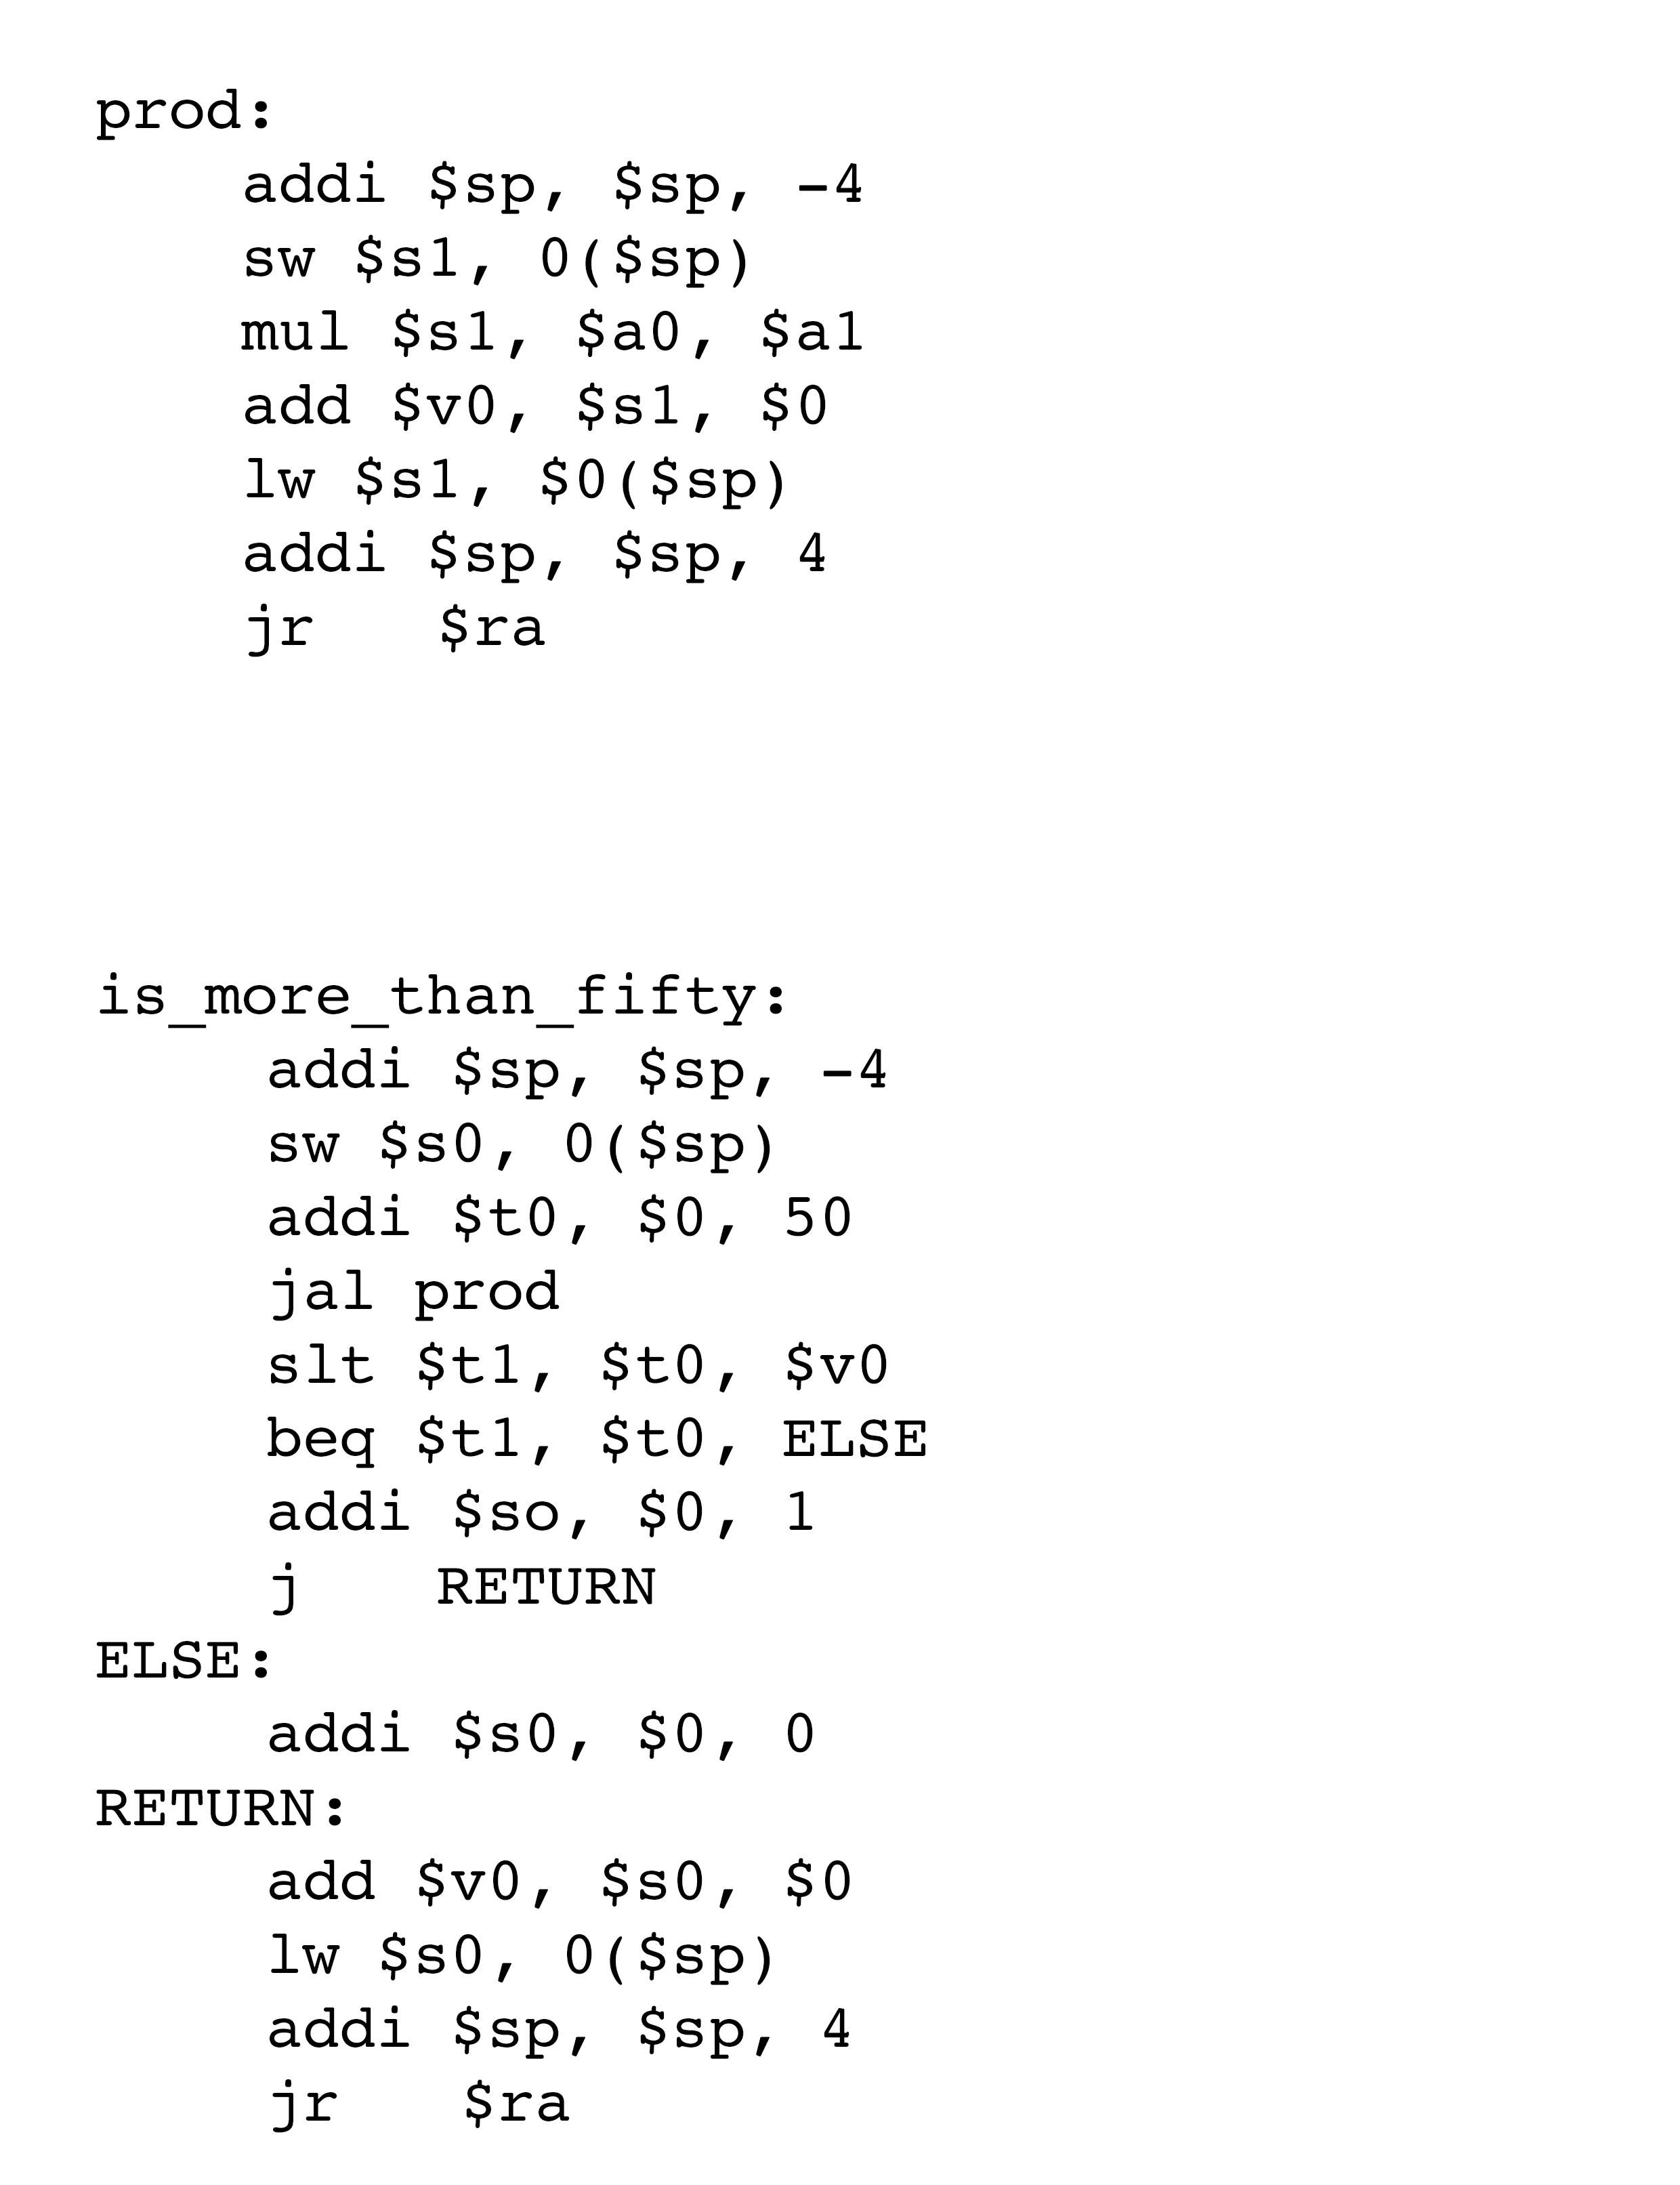
\includegraphics[scale=0.4]{72.png}
\\
$is\_more\_than\_fifty$ function is implemented in mips by first saving space for 1 variable and storing the value 50 in another register. Then the prod function is called and we check with slt if the condition holds. If it doesn't hold, we proceed to the ELSE instructions. The RETURN statement is implemented using the return value \$v0 and jr (jumping back to the scope where the function was called).\\

The instructions in the $prod$ function save space for a variable first, then, the multiplication is done using mul and the return value is put into register \$v0. Space is readjusted and the jump to the scope where the function was called is done using jr.

\pagebreak

\problem{}{0}
\solution

\$s3 = i ; \$s5 = k

\vspace{3mm}


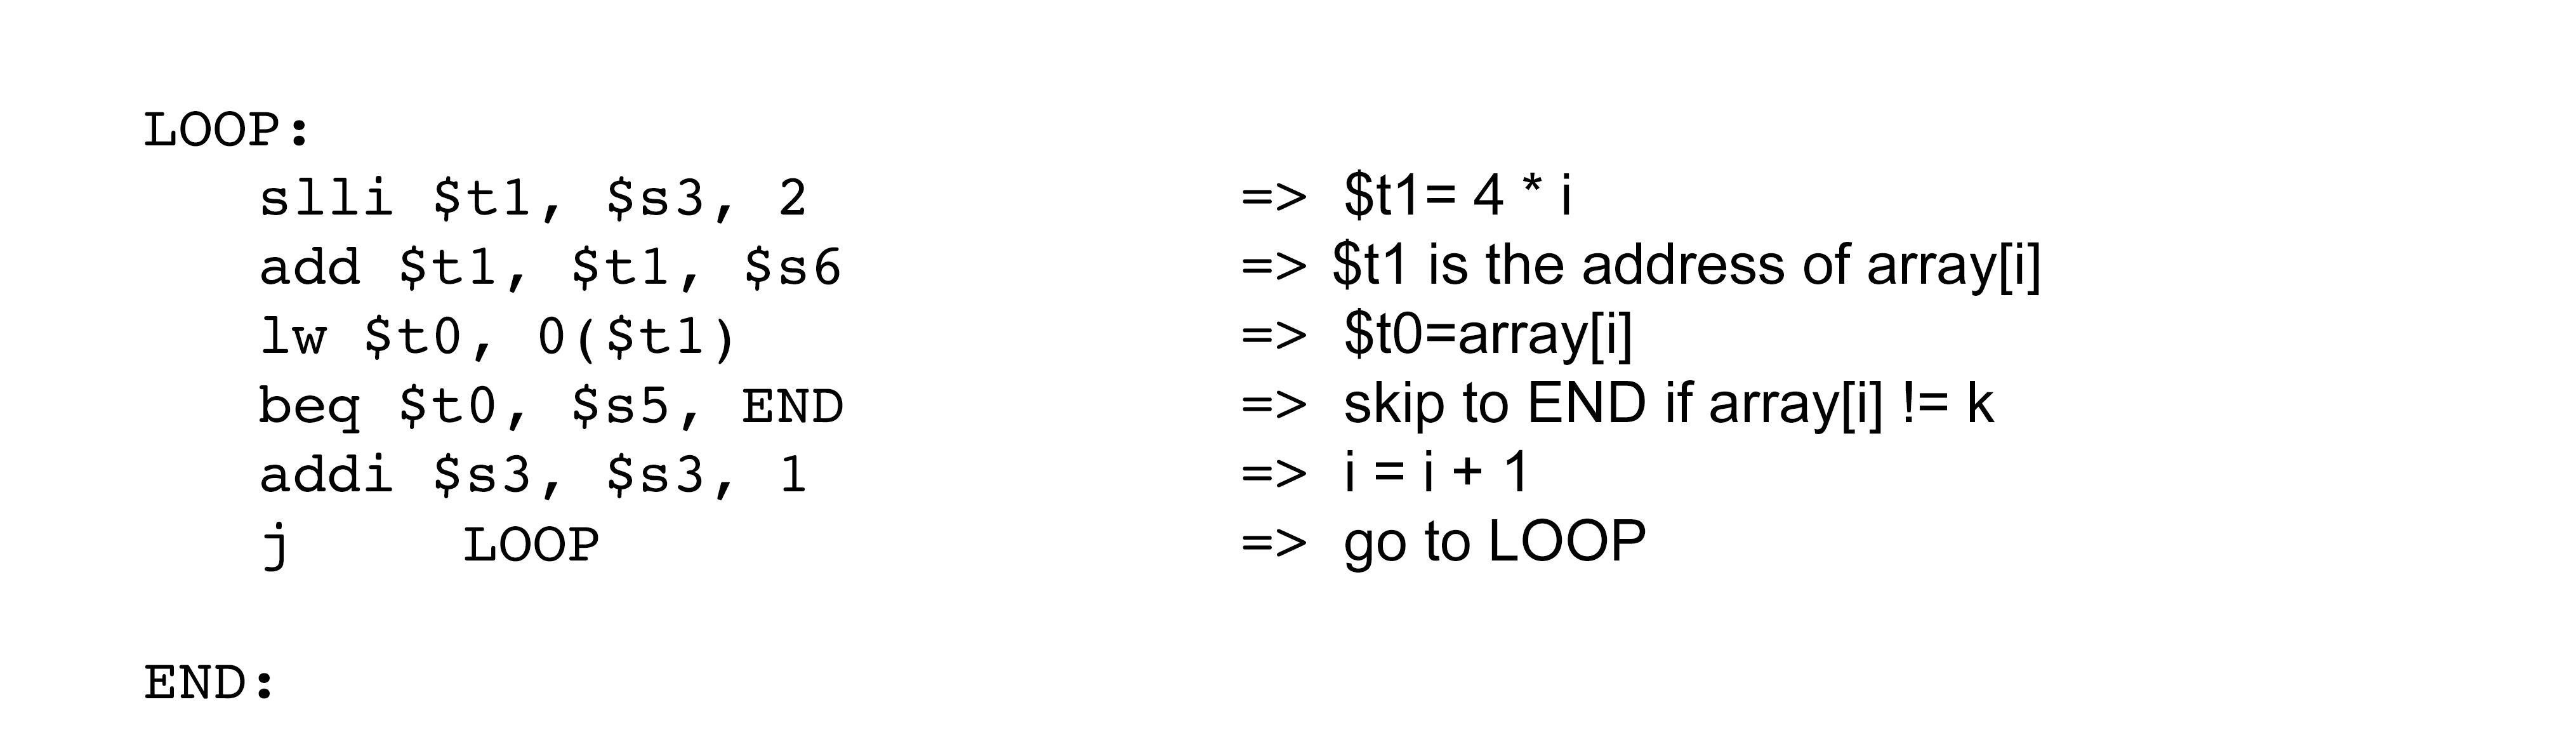
\includegraphics[scale=0.4]{73.png}

\vspace{3mm}

In C code, that can be written in a more simplified way as:\\
${
while (array[i]    !=   -1)}$

$
\qquad i = i + 1
$
\vspace{5mm}
\problem{}{0}
\solution
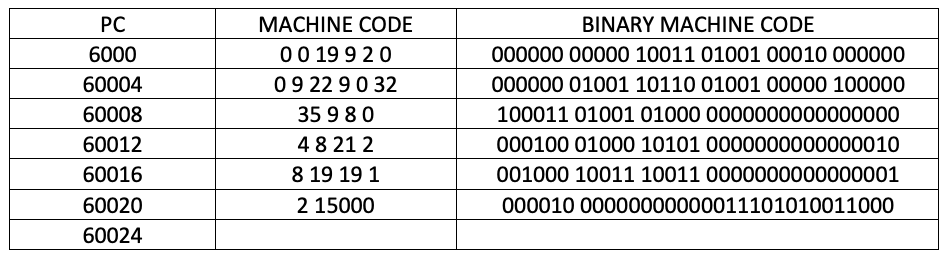
\includegraphics[scale=0.4]{74.png}

\problem{}{0}
\solution
\\
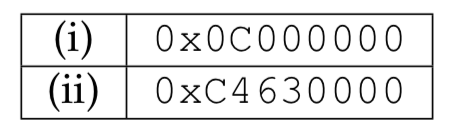
\includegraphics[scale=0.3]{problem5.png}\\
What decimal number does the bit pattern represent:\\
\\
\textbf{a) if it is a two complement number?}\\
\\
(i) 0x0C000000 $= !(0000$ $1100$ $ 0000$ $ 0000$ $ 0000$ $ 0000$ $ 0000$ $ 0000) + 1 = \\
= 1111$ $ 0011$ $ 1111$ $ 1111$ $ 1111$ $ 1111$ $ 1111$ $ 1111 + 1 = 011110100000000000000000000000000 =\\ =-4093640704_{10}$\\
\\
(ii) 0xC4630000 $= !(1100$ $0100$ $0110$ $0011$ $0000$ $0000$ $0000$ $0000) + 1 = \\
= 0011$ $1011$ $1001$ $1100$ $1111$ $1111$ $1111$ $1111 + 1 = 0011$ $1011$ $1001$ $1101$ $0000$ $0000$ $0000$ $0000 = -1000144896_{10}$\\
\\
\textbf{b) if it is an unsigned integer?}\\
\\
(i) 0x0C000000 $ = 0000$ $1100$ $0000$ $0000$ $0000$ $0000$ $0000$ $0000 = 201326592_{10}$\\
\\
(ii) 0xC4630000 $ = 1100$ $0100$ $0110$ $0011$ $0000$ $0000$ $0000$ $0000 = 3294822400_{10}$\\
\\
\textbf{c) if this bit pattern is placed into the Instruction Register, what MIPS instruction would it be?}\\
\\
i) 0x0C000000 $ = 000011$ $00000$ $00000$ $0000000000000000 = $ JAL target\\
\hspace*{8em} op \\
(ii) 0xC4630000 $ = 11000$ $00011$ $00011$ $0000000000000000 = $\\
= op code + base register + destination register + address = \\
= lwc1 \$3, 0(\$3)\\

\end{document}